\documentclass[conference]{IEEEtran}
\usepackage[hyphens,spaces]{url}
\newtheorem{definition}{Definition}
\usepackage{graphicx}
\graphicspath{{./Images/}}
\usepackage{setspace}
\usepackage{subcaption}
\usepackage{algorithm}
\usepackage[noend]{algpseudocode}

\begin{document}

\title{Illinois Tech Basketball Data Analytics}
\author 
{\IEEEauthorblockN{Chenjie Li,Diruba Palabiyik}
\IEEEauthorblockA{Data Science\\
Illinois Institute of Technology\\}
}
\maketitle

\begin{abstract}
In this work, we showcase our approaches and results of our data science practicum project--Illinois Tech Scarlet Hawks Men's Basketball Analysis. Starting from database desgin, we explored some of the most recognized metrics to evaluate players and lineups, such as ``on-off court" data, ``lineup" comparisons, ``offensive and defensive tendencies". Based on our ``scouting reports", our coaching staff made the corresponding strategies and in the end set the best record of our school history.
\end{abstract}

\section{Introduction}

``Analytics are part and parcel of virtually everything we do now." said by NBA commissioner Adam Silver. \\
Data Science, one of the most promising and in-demand career paths for skilled professionals, is expanding its branch to sports. The origin of sports analytics was not basketball. The education begins with the baseball analysis of Bill James \cite{james2010new}. With baseball leading the way, other sports began to embrace data and utilize them to help their teams. Unlike baseball which can be reasonably partitoned into a series of discrete events, basketball is much more complicated and harder to give reasonable analysis. With that being said, there are still a lot of ways to approach this exciting sport and use technology to change the game. In Stephen M. Shea's work \cite{1492923176}, he introduces variety of ways to evaluate players and teams. Also, in  Rajiv's exciting TED talk \cite{tedtalk}, he introduced the implementations of computer vision and machine learning in basketball analytics.\\
As a Division III team, however, the Men's basketball team of Illinois Tech hasn't benefited from this trend due to the lack of available data and technicians.\\
In this program practicum, we built up a database from scratch. Based on that, we explored several branches: Player evaluation, Team evaluation, Lineup Evaluation. Using Tableau software, we got straightforward yet insightful visualizations for coaching staff as references. In the end of the season, we made to the $2nd$ place in the tournament, setting the best record of our school basketball history.

\section{Data Source}
You can't make bricks without straw. Getting data was one of the biggest challenges for us. Thankfully, we were lucky enough to have somethig to work on.
\subsection{Synergy} 
Synergy\cite{synergy} for overall statistics from each player and each team. They provide comprehensive details for players and teams, even the distributions of offensive and defensive tendencies and the corresponding efficiencies. Based on these information, later on we created "strength and weakness", "player clustering" and so on.

\subsection{NACC Official Website}
Another important data source in this project was northern athletics collegiate conference website \cite{nacc}, in which we can get the game ``Play-By-Play" files which can be used for analysis of lineups and ``Player Pairs" analysis.

\section{Database Design}
to do\\

\section{Strength VS Weakness}
There are many ways to evaluate players. One important aspect is ``How efficient is this player?". Here, we chose to use ``Points Per Possession"(ppp) as the measure to differentiate each player's strengths and weaknesses. On Synergy website, it breaks down each player(team)'s offense into different types:\textit{ Spot Up, Transition, Off Screen, Offensive Rebounds, Hand Off, Isolation, Post Up, Miscellaneous}, player(team)'s defense into different types:\textit{ Spot Up, Off Screen, P\&R Ball Handler, Hand Off, Isolation, Post-Up, P\&R Roll Man}. for each type, Synergy collects and computes its corresponding \textit{Percentage of time}, which is basically the frequency of this player's all offensive(defensive) types. Also, it lists the points per possesion, which is showing how many point(s) this player can score in each offensive (or how many point(s) this player's opponent can score in each offensive possesion). 

\begin{definition}[Strengh and Weakness]
Given a player's offensive average $ppp_{off\_overall}$, the strength for the player is $ppp_{off\_strength}>ppp_{off\_overall}$, the weakness for the player is $ppp_{off\_weakness}<ppp_{off\_overall}$; Given a player's defensive average $ppp_{def\_overall}$, the strength for the player is $ppp_{def\_strength} < ppp_{def\_overall}$, the weakness for the player is $ppp_{def\_weakness}<ppp_{def\_overall}$.
\end{definition}

The reason for choosing `` $ppp_{def\_strength} < ppp_{def\_overall}$" is that it shows how good this player is in making his opponent inefficient.

For this part, we store those information in \textit{``player(team) average"} table

We chose 2 different ways of showing the visualizations in Tableau. The first one, Fig ~\ref{fig:S-and-W-1} is showing the distributions of each player's play types. It has different filters on this dataset. For example, users can filter based on team,offensive/defensive, player etc. Fig ~\ref{fig:S-and-W-2} is showing in a more straightforward way. The red reference line is player's $ppp_{overall}$.

\begin{figure}
  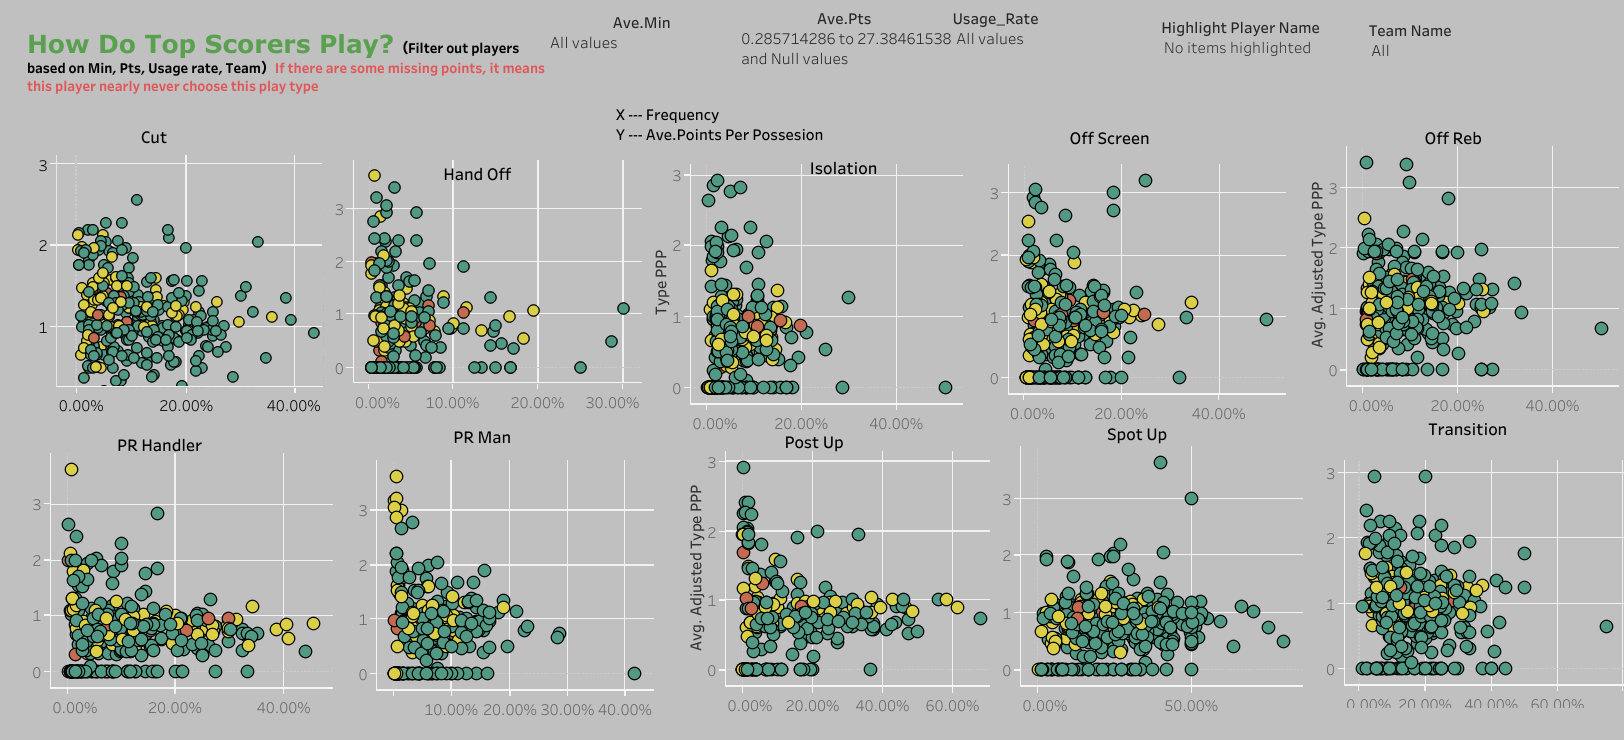
\includegraphics[width=\linewidth]{Strength_Weakness.jpg}
  \caption{Strength and Weakness 1}
  \vspace{-1mm}
  \label{fig:S-and-W-1}
\end{figure}

\begin{figure}
  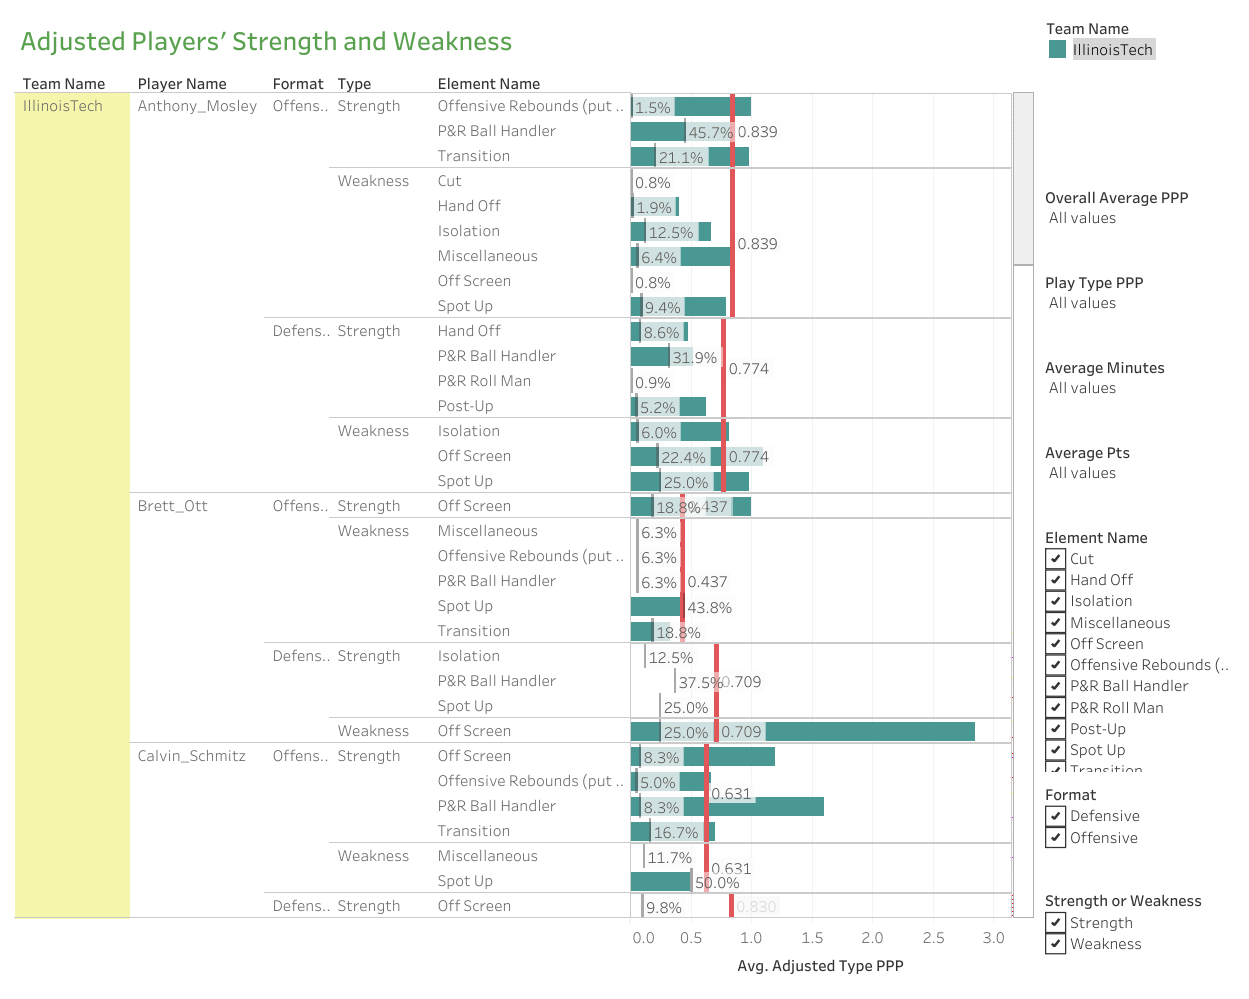
\includegraphics[width=\linewidth]{Strength_Weakness_2.jpg}
  \caption{Strength and Weakness 2}
  \vspace{-1mm}
  \label{fig:S-and-W-2}
\end{figure}

\section{Lineup Anaysis}
In this section, we essentially did 2 things, ``individual player's contribution" to team and ``pairs' performance". The reason why we consider both of these 2 aspects are: A player might be normal or average when evaluated individually, but his ``pair" with some other teammates may give us an surprising result(pairwise); At the same time, we do need individual player's performance as a reference to be able to give ourselves a sense of what kind of a player is. For instance, consider ``Plus Minus" as the measuring metric, player A's personal plus minus is +100 in the season, whereas his average plus minus with other teammates together(pairs) is only +10. this could give us 2 insights: player A is very good; he might need to work on involving his teammates. We do admit that this is not necessarily true. For example, A is just in another level compared with his teammates, we can't jump to the conclusion like this solely based on one metric.

With the idea above, there's actually a lot more we should do: we didn't have the stats in that detail. For example, to get the ``pairwise performance", we need to get the stats only when those pairs were on the court. But we didn't have those at hand.

Thankfully, we finally found something to get started. Nowadays, most basketball games' broadcasting service will feature a section called ``play-by-play", which is a document- like file that will keep what happened on the court in it. So we decided to write a program that can process it and generate the stats we want. A sample of ``play-by-play" file: \\
($www.illinoistechathletics.com/sports/mbkb/2018\-19/boxscores/20190223\_a3e3.xml?view=plays$)

\begin{figure}[h!]
  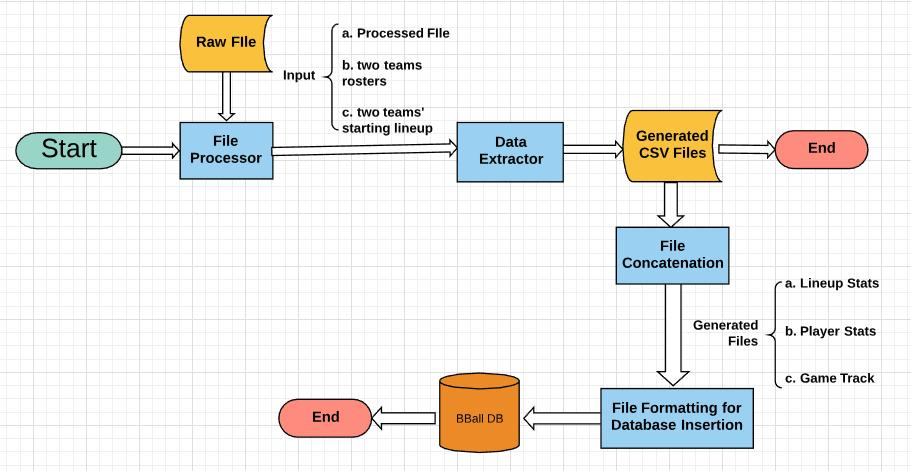
\includegraphics[width=\linewidth]{flowchart.jpg}
  \caption{Program Pipeline}
  \vspace{-1mm}
  \label{fig:flowchart}
\end{figure}

Fig ~\ref{fig:flowchart} shows the flow of our designed program. $\bf{Raw\;File}$ is just ``Play-By-Play" file which we can easily get just using traditional ``Copy and Paste" action(Ctrl+A in the website and Ctrl+C, Ctril+V to a .txt file). $\bf{File\;Processor}$ is a program that can handle some special structural problems in raw file, like cleaning up a miscellaneous collection of redundant data and strange time sequence (some incorrect sequence of the game timeline).$\bf{Data\; Extractor}$ is the main part of the program. when using this program, user needs to specify the starting lineups of both teams, and we made the assumption that for both first and second half, both teams were using the same lineups. In reality, of course, this is a bad assumption, but user can manually change the input in the program if there's any changes in the starting lineups in the second half. After running the program, it will generate 3 files: $\textit{Lineup Stats, Player Stats, Game Track}$. $\textit{Lineup Stats}$ contains the stats for the whole lineup (5 players combined). It also has the corresponding stats for the opponent stats.$\textit{Lineup Stats}$ were saved in $Lineup$ Table of our database.$\textit{Player Stats}$ contains each individual player's stats in each different lineup, i.e. $Player A$'s stats in Lineup $a$ is a row of data, whereas $Player A$'s stats in Lineup $b$ is another row of data.$\textit{Player Stats}$ were saved in $Player\_Game$ Table of our database. $\textit{Game Track}$ is a file that records the change of the score difference between two teams as time changes.$\textit{Game Track}$ data were saved in $Game\_Track$ Table of our database.In $\bf{File\;Concatenation}$, in the case of generating files for multiple games at once, we might want to concatenate them together before formatting them in the next step. In $\bf{File\;Formatting\;For\;Database\;Insertion}$, we map the field names into the $\textit{keys}$ in the database tables we created.

After all these steps above, we finally got the stats we need to perform the analysis we want in the first place.

For the rest of the section, we will discuss the algorithm we used for generating $\textbf{Top-K}$ pairs for each player in terms of the given metric.

\begin{definition}[Top-K Pairs]
Given the direction of the metric $\theta \in \{high,low\}$, the measuring metric $\sigma$, player $P$, $P_{\sigma,\theta}^k$ is a set of players that are best $K$ pairs with this player $P$.
\end{definition}

\begin{algorithm}
\caption{Top-K pairs}\label{euclid}
\label{alg:topk}
\begin{algorithmic}[1]
\State $R \gets \textit{the set of all the players in the team (Rosters)}$
\State $p_0 \gets \textit{target player}$
\Procedure{Top-K generation}{$R$, $\theta$, $\sigma$,$p_0$}

\For {each p in R}
  \If {$p == p_0$}
    \State $\textit{Continue}$
  \Else
    \State $\textit{Candidate\_Pair} \gets SORT\{p,p_{0}\}$
    \If{$\theta == low$}
      \State $heap \gets MinHeap$
    \Else
      \State $heap \gets MaxHeap$
    \EndIf
    \State $\textit{Q =}$ 
    \State $\textit{SELECT p as target\_player, Candidate\_Pair as }$
    \State $\textit{pair,$\sigma$ as metric FROM Lineup}$
    \State $\textit{WHERE lineup\_players like \%Candidate\_Pair\%}$
    \State $result \gets R(Q)$
    \If {$\textit{heap.size $<$ K}$}
      \State $\textit{heap.insert(result)}$
    \ElsIf{$ heap.peek (\leq if\;minheap\;or\geq\;if\;maxheap)\; result$}
      \State $\textit{heap.insert(result)}$
    \EndIf
\EndIf
\EndFor
\EndProcedure
\end{algorithmic}
\end{algorithm}
In the Algorithm ~\ref{alg:topk}, we ignored the number of players in each pair, i.e. we treat ``2-men" pair and ``3-men" pairs the same way. Combine those work together, we generated the visualization for pairs and individual ``On and Off court" using ``Plus Minus" as our evaluating metric as shown in Fig ~\ref{fig:pairs}
\begin{figure}[h!]
  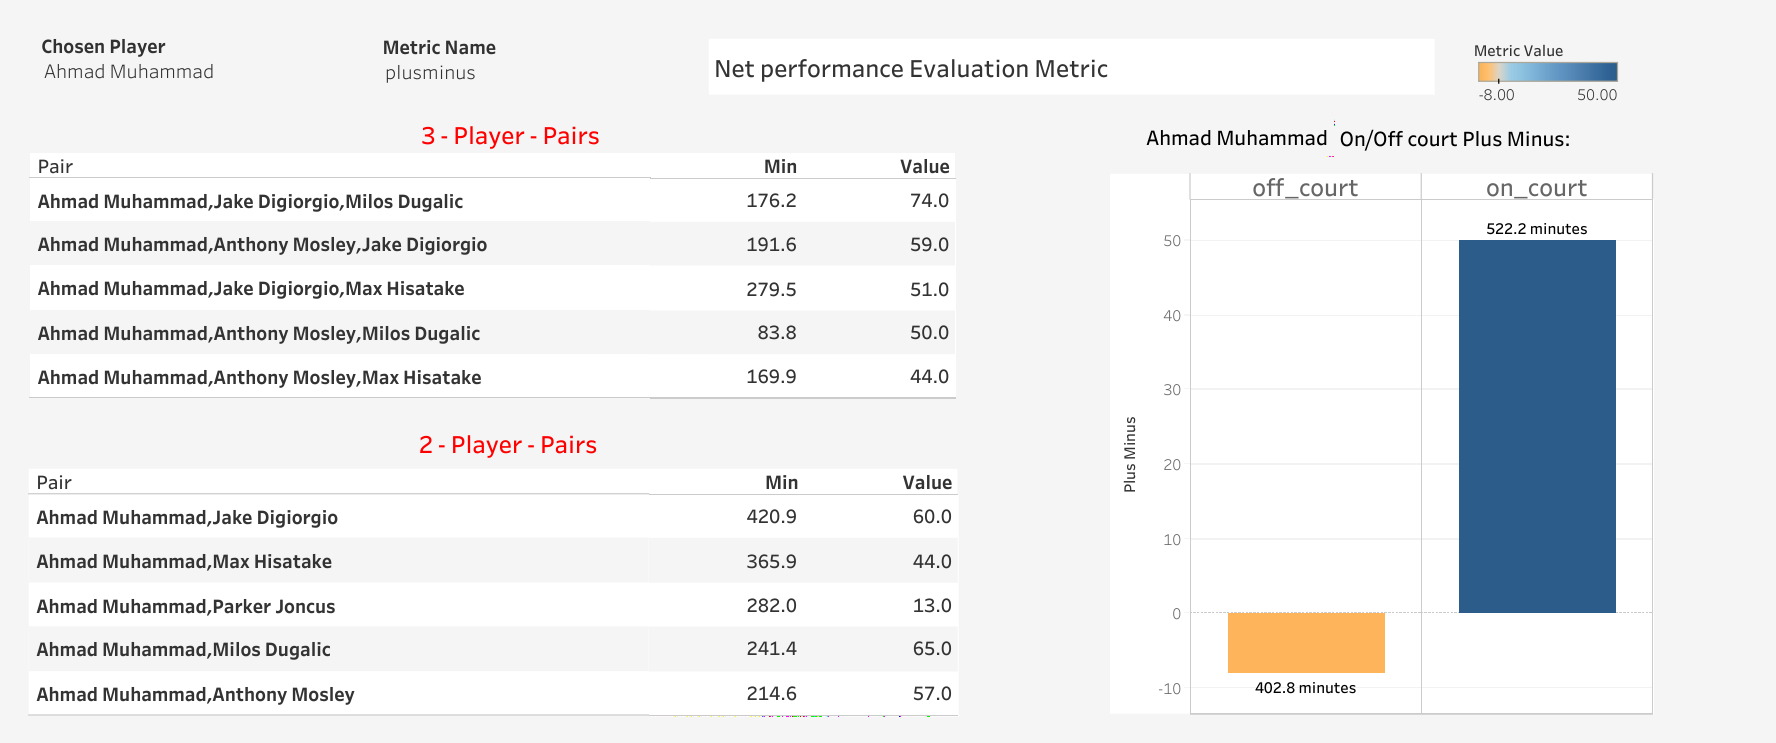
\includegraphics[width=\linewidth]{pairs.jpg}
  \caption{Pairwise and Individual Plus Minus}
  \vspace{-1mm}
  \label{fig:pairs}
\end{figure}

\begin{figure}[h!]
  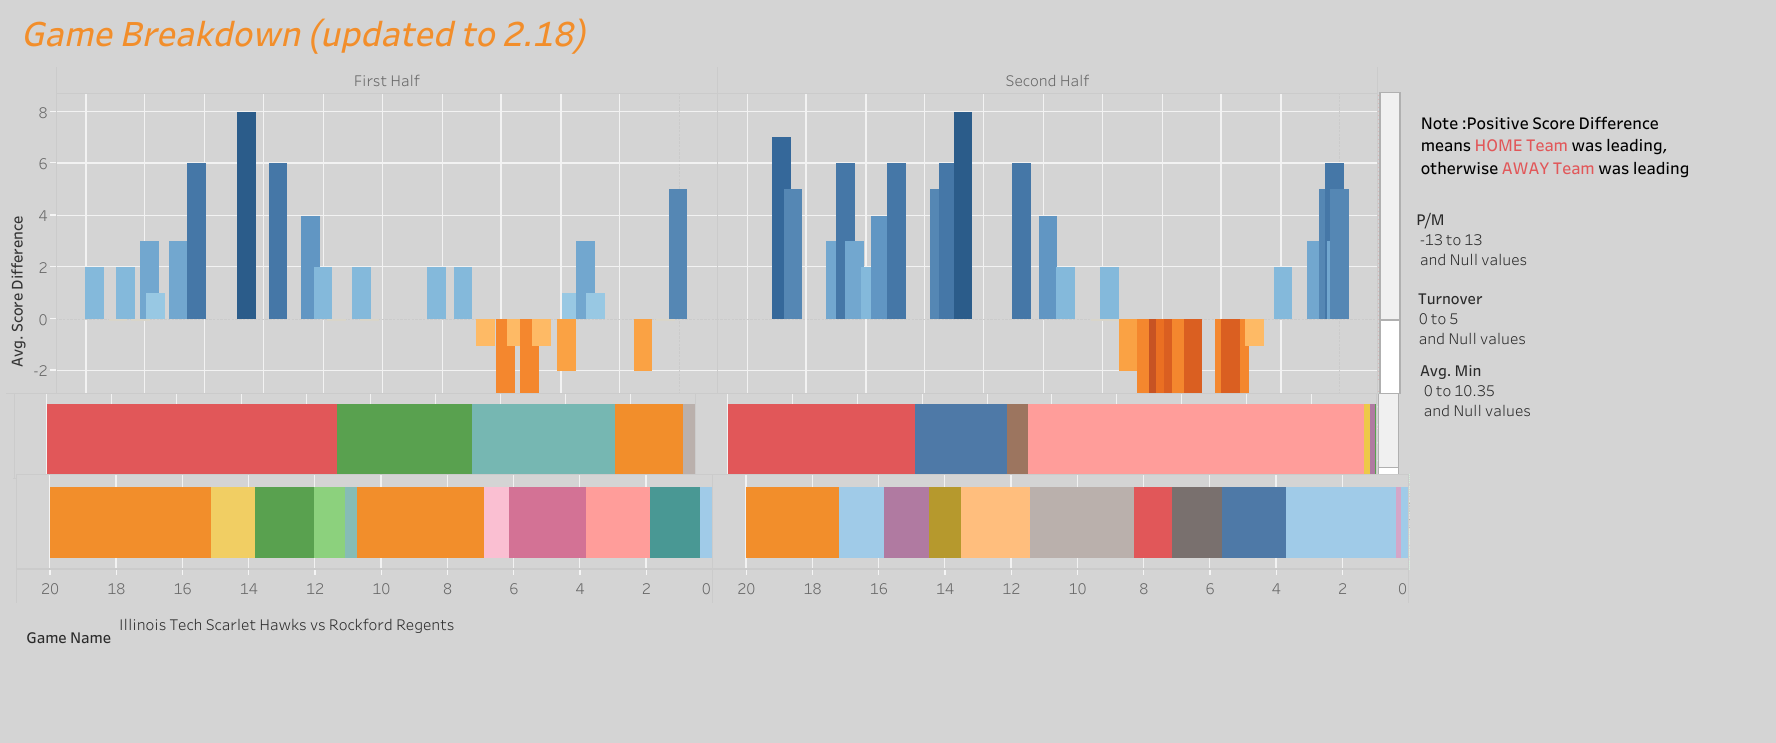
\includegraphics[width=\linewidth]{gameflow.jpg}
  \caption{Game Flow Visualization}
  \vspace{-1mm}
  \label{fig:gameflow}
\end{figure}
By implementing the data from $Game\_Track$ Table, we generated the ``Game Flow" chart as shown in Fig \. Different colors means the different lineups and the barchart above are the score differences between 2 teams.

Besides, after our team made to the tournament, we came up with a ``scouting report" by combining the strength and weakness in section IV with the play-by-play data to give our coach a more efficient and more convenient way to study our opponents. One example of the ``Scouting Report" is shown in Fig \ref{fig:scouting}
\begin{figure}[h!]
  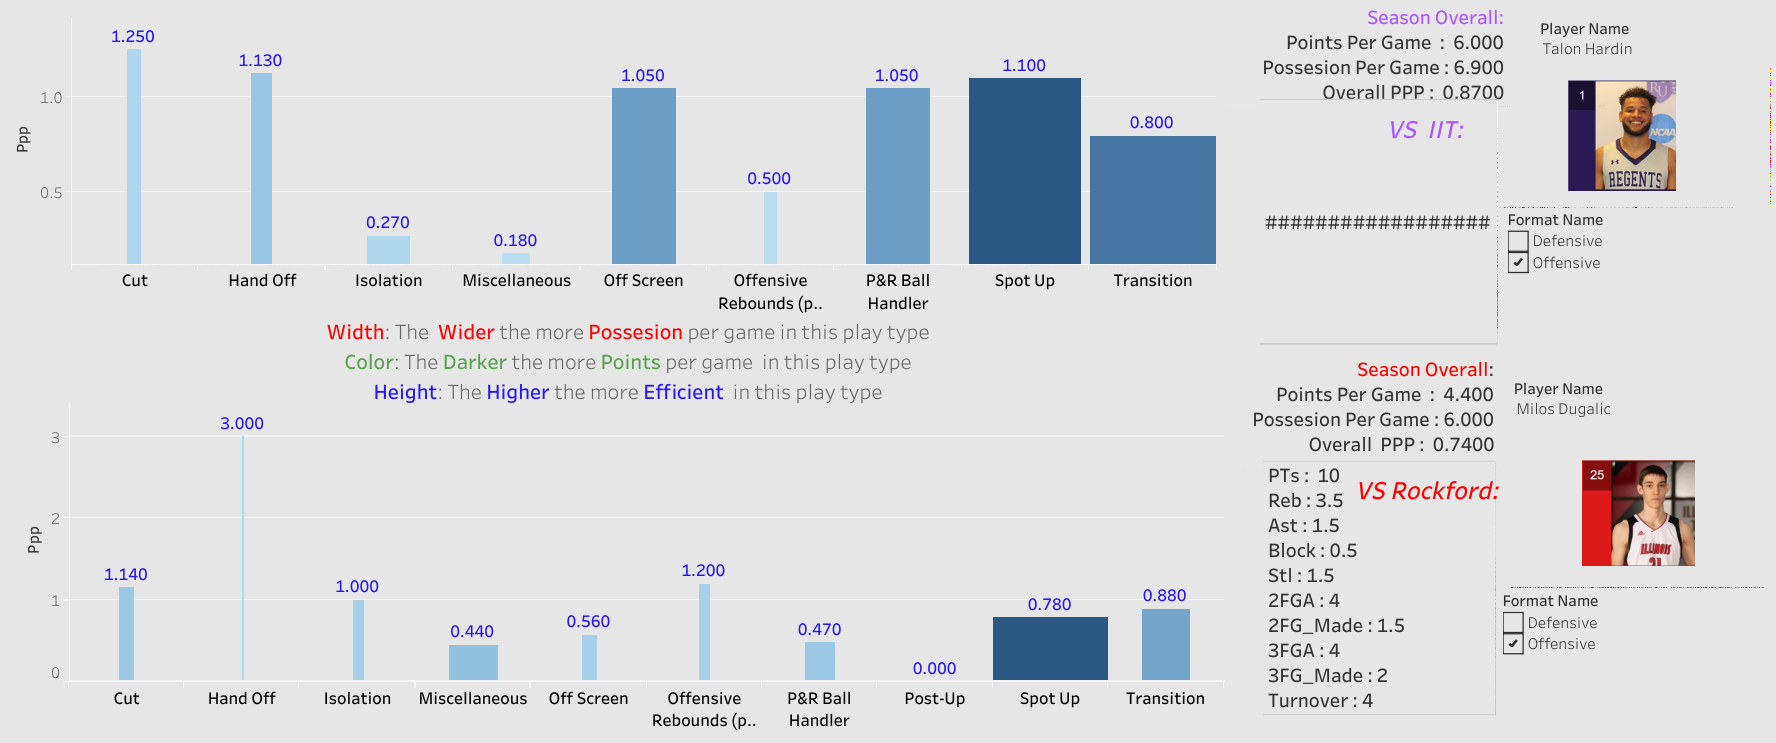
\includegraphics[width=\linewidth]{scouting.jpg}
  \caption{Sample Scouting Report}
  \vspace{-1mm}
  \label{fig:scouting}
\end{figure}

\clearpage
\bibliographystyle{unsrt}
\bibliography{references}
\end{document}

